\documentclass[11pt,letterpaper,final]{report}
\usepackage[utf8]{inputenc}
\usepackage[francais]{babel}
\usepackage[T1]{fontenc}
\usepackage{amsmath}
\usepackage{amsfonts}
\usepackage{amssymb}
\usepackage{graphicx}
\usepackage{lmodern}
\usepackage[left=2.54cm,right=2.54cm,top=2.54cm,bottom=2.54cm]{geometry}
\begin{document}
\chapter{Cross validation entre les différentes plateformes de simulations}
\section{Validation Psim/SPS}
\begin{figure}[ht]
\centering
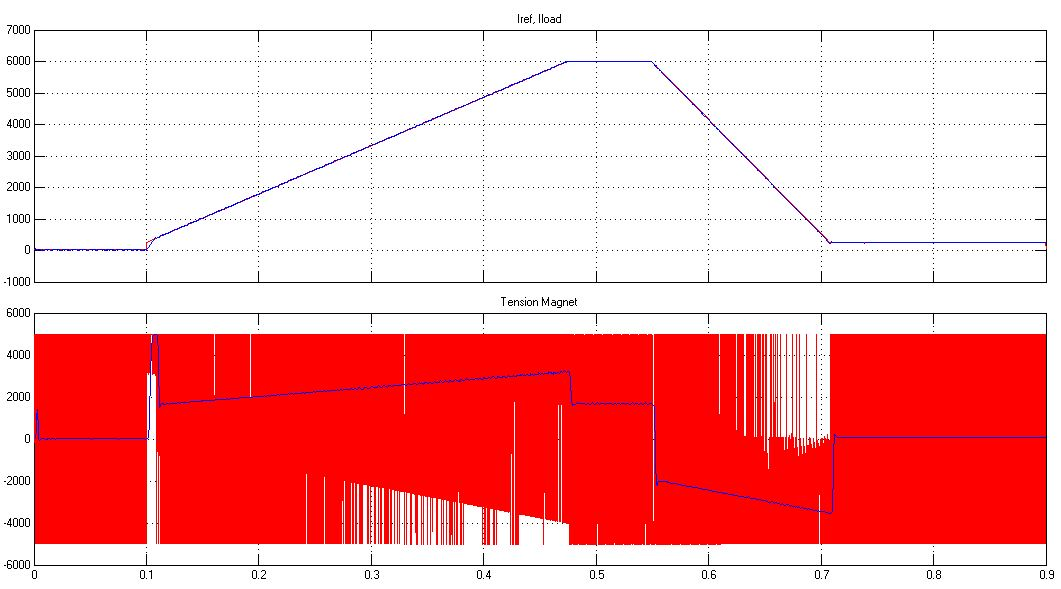
\includegraphics[scale=0.5]{fig/resul_sim.jpg}
\caption{Résultats de simulation sur SIMULINK}
\end{figure}
\begin{figure}[ht]
\centering
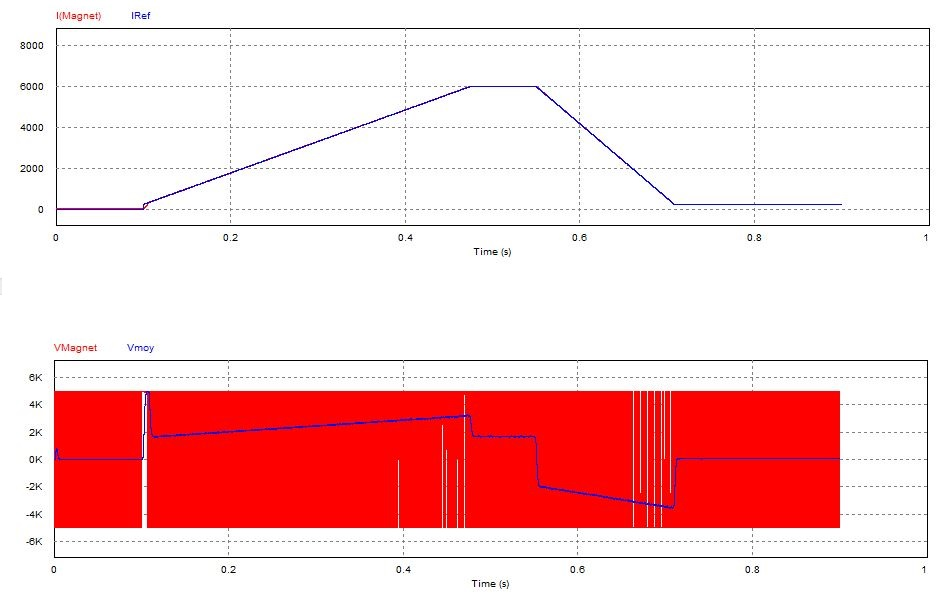
\includegraphics[scale=0.6]{fig/resul_psim.jpg}
\caption{Résultats de simulation sur Psim}
\end{figure}
\subsection{Calcul de la tension moyenne}

Commençons par discuter des différences obtenues entre les différentes simulations. On a remarqué que la fonction "Mean" dans simulink et Psim ne donne pas le même résulat. Pour le montrer, on a testé chacune des deux fonctions avec un sinus 100Vamplitude, 50Vmoy et à 1KHz de fréquence. Les figures~\ref{dis_mean} et \ref{D_mean} montre les résulats obtenus avec une fréquence de 500Hz du moyenneur.



\begin{figure}[h]
\centering
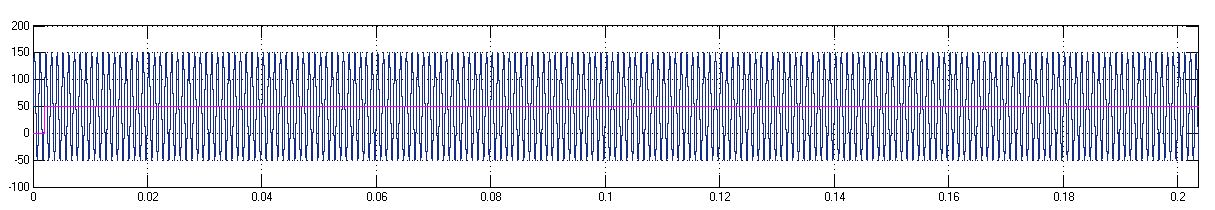
\includegraphics[scale=0.5]{fig/moy_sim.jpg}
\caption{Réponse de la function "Discrete Mean" sur SPS}
\label{dis_mean}
\end{figure}

\begin{figure}[h]
\centering
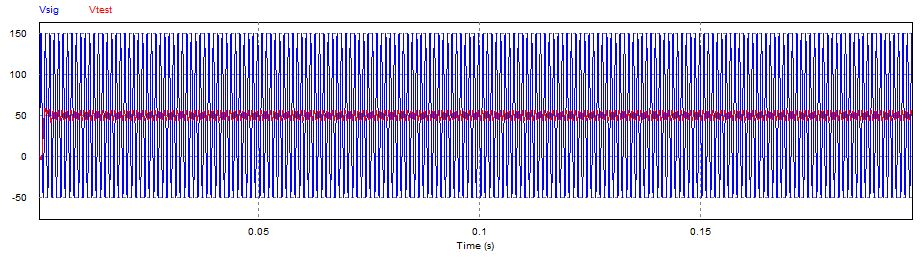
\includegraphics[scale=0.5]{fig/moy_psim.jpg}
\caption{Réponse du bloc "DC Voltmeter" sur PSIM}
\label{D_mean}
\end{figure}


\begin{figure}[ht]
\centering
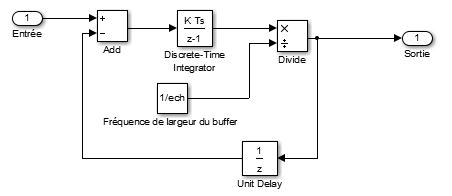
\includegraphics[scale=0.8]{fig/moy.jpg}
\caption{Fonction de moyennage de la tension}
\label{moy}
\end{figure}
On remarque bien que les résultats sont différents dans les figures~\ref{dis_mean} et \ref{D_mean}. La tension moyenne calculé sur simulink est plus précise  et varie moins que celle de Psim. La précision est telle que le résultat de Psim est variant sur chaque période tandis que celle de simulink a une apparence droite. Par contre, le temps de réponse de simulink est plus long que celui de Psim. Par conséquent, on a décidé de monter notre propre fonction de moyennage pour avoir un fonctionnement identique dans les deux simulations. La figure~\ref{moy} représente la fonction qui est constitué d'un intégrateur avec un gain unitaire. Cette valeur est passé dans un gain de 3000 qui contrôle la sensibilité du calcul de moyennage. De plus, on a cascadé 10 fonctions de moyennage pour optimiser le résultat et avoir une moyenne avec une oscillation négligeable. Les filtres donnent le même résultat sur les deux plateformes donc le fonctionnement de la fonction de moyennage sur Psim donne le même résulat que celle de Simulink si le signal d'entrée est le même. 






\begin{figure}[h!]
\centering
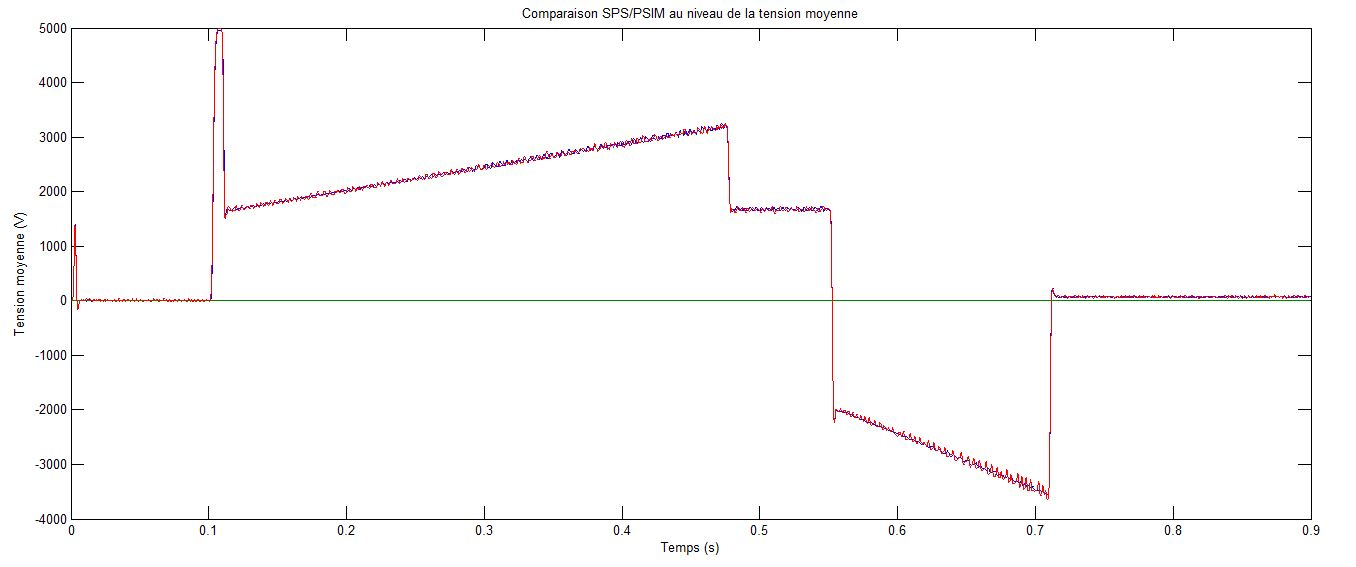
\includegraphics[scale=0.4]{fig/tmoypsim_sim.jpg}
\caption{La tension moyenne Psim/Simulink}
\label{moyt}
\end{figure}
Sur la figure~\ref{moyt} on capte la différence relative entre la tension moyenne sur Psim et Simulink. La courbe en rouge représente la réponse sur Psim et en bleu celle sur Simulink. La différence observé est dû au fait que sur Simulink nous utilisons des IGBT idéaux donc qui commutent instantanément, tandis que sur Psim ce sont des IGBT qui ont un temps de commutation faible mais non négligeable. Leur modélisation ne sont pas pareil, Simulink les a modéliser comme des interrupteurs idéaux tandis que Psim les a modéliser comme des interrupteurs non-idéaux. De sorte que, c'est normal qu'on n'a pas le même résultat car la simulation de Psim à une perte de commutation tandis que celle de Simulink n'en contient pas. Mais, on constate que les résultats sont très semblables avec une erreur moyenne de seulement 0.16\% calculé selon l'équation~\ref{eq1}.
\begin{equation}
Erreur = \frac{mean(V_{moy Simulink})-mean(V_{moy Psim})}{mean(V_{moy Simulink})}
\label{eq1}
\end{equation}

On constate que Psim ne peut pas avoir un pas de calcul de $10^{-6}$. À cause de la complexité de la simulation, SimView n'est plus capable de s'exécuter à cause d'un manque de mémoire. Pour Simulink, le pas de calcul doit être à $10^{-5}$ si on veut garder une fréquence de commutation à 1 Khz vu sur la charge. La fréquence de commutation varie en fonction du pas de calcul.


\subsection{Calcul du courant}
Nous avons comparés les deux plateformes concernant la différence obtenus au niveau du courant de charge. Nous avons obtenu une différence de 0.011\%
entre Psim et Simulink en utilisant la valeur moyenne de courant pour le calcul en suivant l'équation~\ref{eq2}. On déduit donc que la simulation de Psim représente le fonctionnement réel du système car il reproduit bien les résultats obtenus sur Simulink .
 
\begin{equation}
Erreur = \frac{mean(I_{simulink})-mean(I_{Psim})}{mean(I_{simulink})}
\label{eq2}
\end{equation}


\begin{figure}[ht]
\centering
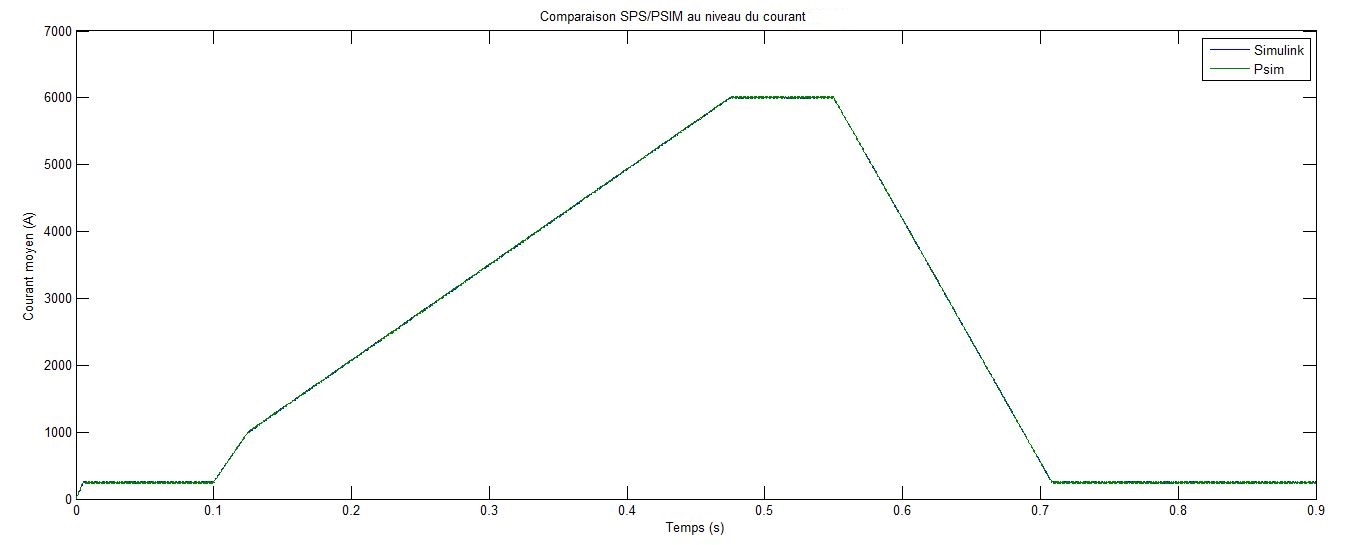
\includegraphics[scale=0.5]{comp_PSIM_SPS.jpg}
\caption{L'erreur entre PSIM et SPS}
\label{comp_PSIM_SPS}
\end{figure}



\end{document}